\documentclass[11pt, dvipsnames, handout]{beamer}
\newtoggle{full}
\settoggle{full}{true}

\newtoggle{covered}
\settoggle{covered}{false}

\newtoggle{presentable}
\settoggle{presentable}{false}

\newtoggle{dualscreen}
\settoggle{dualscreen}{false}

\usepackage{pgfplots}
%\pgfplotsset{compat = newest}

\usepackage{pgfpages}

\setbeamertemplate{note page}{\pagecolor{yellow!5}\vfill \insertnote \vfill}
\usepackage{collect}
\definecollection{notes}
\newcounter{notestaken}

\usepackage{xpatch}

\usepackage{ulem}

\usepackage[framemethod=tikz]{mdframed}

\usepackage{scalerel}
\usepackage{calc}

%\usepackage{enumitem}
\setlength\fboxsep{.2em}

\usepackage{graphicx} % Allows including images
\usepackage{booktabs} % Allows the use of \toprule, \midrule and \bottomrule in tables

\xpatchcmd{\itemize}
  {\def\makelabel}
  {\setlength{\itemsep}{0.65 em}\def\makelabel}
  {}
  {}


\xpatchcmd{\beamer@enum@}
  {\def\makelabel}
  {\setlength{\itemsep}{0.65 em}\def\makelabel}
  {}
  {}


%\makeatletter
%\renewcommand{\itemize}[1][]{%
%  \beamer@ifempty{#1}{}{\def\beamer@defaultospec{#1}}%
%  \ifnum \@itemdepth >2\relax\@toodeep\else
%    \advance\@itemdepth\@ne
%    \beamer@computepref\@itemdepth% sets \beameritemnestingprefix
%    \usebeamerfont{itemize/enumerate \beameritemnestingprefix body}%
%    \usebeamercolor[fg]{itemize/enumerate \beameritemnestingprefix body}%
%    \usebeamertemplate{itemize/enumerate \beameritemnestingprefix body begin}%
%    \list
%      {\usebeamertemplate{itemize \beameritemnestingprefix item}}
%      {%
%        \setlength\topsep{1em}%NEW
%        \setlength\partopsep{1em}%NEW
%        \setlength\itemsep{1em}%NEW
%        \def\makelabel##1{%
%          {%
%            \hss\llap{{%
%                \usebeamerfont*{itemize \beameritemnestingprefix item}%
%                \usebeamercolor[fg]{itemize \beameritemnestingprefix item}##1}}%
%          }%
%        }%
%      }
%  \fi%
%  \beamer@cramped%
%  \raggedright%
%  \beamer@firstlineitemizeunskip%
%}
%
%
%
%
%
%\makeatother

%\setlist[beamer@enum@]{topsep=1 em}
%\let\origcheckmark\checkmark %screw you dingbat
%\let\checkmark\undefined %screw you dingbat
%\usepackage{dingbat} 
%\let\checkmark\origcheckmark %screw you dingbat






%\usepackage{fontawesome}

\usepackage{mathtools}
\usepackage{etoolbox, calculator}

\usepackage{xcolor}
\usepackage{tikz}
\usetikzlibrary{arrows.meta}
\usetikzlibrary{calc}
\usepackage[nomessages]{fp}
\usepackage{transparent}
\usepackage{accsupp}
%\usepackage{color, xcolor}

%colorblind-friendly palette
%\definecolor{dblue}{RGB}{51,34,136}
\definecolor{lblue}{RGB}{136,204,238}
%\definecolor{green}{RGB}{17,119,51}
\definecolor{tan}{RGB}{221,204,119}
%\definecolor{mauve}{RGB}{204,102,119}

\usepackage{tcolorbox}



\usepackage{xifthen}
\usepackage{nicefrac}
\usepackage{amsmath}
\usepackage{amsthm}
\usepackage{amssymb}
\theoremstyle{definition}
\newtheorem*{define}{Definition}
\newtheorem*{recall}{Recall}


\DeclareMathOperator{\tr}{tr}

\usepackage{multicol}
%\setlength{\columnsep}{1cm}

\usepackage{tablists, amsmath,vwcol, cancel, polynom}
\usetikzlibrary{shapes, patterns, decorations.shapes}
%\usepackage{tikzpeople}
\tikzstyle{vertex}=[shape=circle, minimum size=2mm, inner sep=0, fill]
\tikzstyle{opendot}=[shape=circle, minimum size=2mm, inner sep=0, fill=white, draw]

% common math quick commands
\newcommand{\nicedd}[2]{\nicefrac{\text{d}#1}{\text{d}#2}}
\newcommand{\dd}[2]{\dfrac{\text{d}#1}{\text{d}#2}}
\newcommand{\pd}[2]{\dfrac{\partial #1}{\partial#2}}
\renewcommand{\d}[1]{\text{d}#1}
\newcommand{\ddn}[3]{\dfrac{\text{d}^{#3}#1}{\text{d}#2^{#3}}}
\newcommand{\pdn}[3]{\dfrac{\partial^{#3}#1}{\partial#2^{#3}}}
\newcommand{\p}[0]{^{\prime}}
\newcommand{\pp}[0]{^{\prime\prime}}
\newcommand{\op}[2][\text{L}]{#1 \left[ #2 \right]}

\newcommand{\lap}[1]{\mathcal{L}\left\{#1\right\}}
\newcommand{\lapinv}[1]{\mathcal{L}^{-1}\left\{#1\right\}}
\newcommand{\lapint}[1]{\int_0^\infty e^{-st}#1dt}
\newcommand{\evalat}[2]{\Big|_{#1}^{#2}}

\newcommand{\paren}[1]{ \left( #1 \right)}

\newcommand{\haxis}[4][\normcolor]{\draw[#1, <->] (-#2,0)--(#3,0) node[right]{$#4$}; }


\newcommand{\axis}[4]{\draw[\normcolor, <->] (-#1,0)--(#2,0) 
node[right]{$x$};
\draw[help lines, <->] (0,-#3)--(0,#4) node[above]{$y$};}

\newcommand{\laxis}[6]{\draw[<->] (-#1,0)--(#2,0) 
node[right]{$#5$};
\draw[ <->] (0,-#3)--(0,#4) node[above]{$#6$};}
\newcommand{\xcoord}[2]{
	\draw (#1,.2)--(#1,-.2) node[below]{$#2$};}
\newcommand{\textnode}[3]{
	\draw (#1,#2) node[below]{$#3$};}
	
\newcommand{\nxcoord}[2]{
	\draw (#1,-.2)--(#1,.2) node[above]{$#2$};}
\newcommand{\ycoord}[2]{
	\draw (.2,#1)--(-.2,#1) node[left]{$#2$};}
\newcommand{\nycoord}[2]{
	\draw (-.2,#1)--(.2,#1) node[right]{$#2$};}
\newcommand{\dlim}{\displaystyle\lim}
\newcommand{\dlimx}[1]{\displaystyle\lim_{x \rightarrow #1}}
\newcommand{\stickfig}[2]{
	\draw (#1,#2) arc(-90:270:2mm);
	\draw (#1,#2)--(#1,#2-.5) (#1-.25,#2-.75)--(#1,#2-.5)--(#1+.25,#2-.75) (#1-.2,#2-.2)--(#1+.2,#2-.2);}	

%\newcounter{example}
%\setcounter{example}{1}
%\newcounter{preFrameExample}
%\AtBeginEnvironment{frame}{\setcounter{preFrameExample}{\value{example}}}
%\newcommand{\ex}[1]{
%	 \setcounter{example}{\value{preFrameExample}}
%	 \textcolor{green}{\small\fbox{Example \arabic{example}: #1}}\\[8pt]
%	\stepcounter{example}}
%\newcommand{\exans}[1]{
%	\SUBTRACT{\value{preFrameExample}}{1}{\n}
%	 \textcolor{green}{\small\fbox{Solution \n: #1}}\\[8pt]}
\mode<presentation> {

% The Beamer class comes with a number of default slide themes
% which change the colors and layouts of slides. Below this is a list
% of all the themes, uncomment each in turn to see what they look like.


\usetheme{CambridgeUS}
\usecolortheme[named=black]{structure}


\newcommand{\studentcolor}[0]{ForestGreen}
\newcommand{\normcolor}[0]{NavyBlue}
\newcommand{\alertcolor}{Red}

\setbeamercolor{normal text}{fg=\normcolor}
\setbeamercolor{frametitle}{fg=\normcolor}
\setbeamercolor{section in head/foot}{fg=Black, bg=Gray!20}
\setbeamercolor{subsection in head/foot}{fg=Green!70!Black, bg=Gray!10}
\setbeamercolor{alerted text}{fg=\alertcolor}
\setbeamerfont{alerted text}{series=\bf}
\setbeamertemplate{enumerate items}[default]
\setbeamercolor{enumerate item}{fg=\normcolor}

\setbeamertemplate{footline} % To remove the footer line in all slides uncomment this line
%\setbeamertemplate{footline}[page number] % To replace the footer line in all slides with a simple slide count uncomment this line

\setbeamertemplate{navigation symbols}{} % To remove the navigation symbols from the bottom of all slides uncomment this line
}

\newcommand{\alertbox}[1]{\tcbox[on line, colframe=\alertcolor, colback=White, left=2pt,right=2pt,top=2pt,bottom=2pt]{\usebeamercolor*{normal text}#1}}


\newcommand{\startstu}{\setbeamercolor{normal text}{fg=\studentcolor}\usebeamercolor*{normal text}\setbeamercolor{enumerate item}{fg=\studentcolor}\usebeamercolor*{enumerate item}}
\newcommand{\stopstu}{\setbeamercolor{normal text}{fg=\normcolor}\usebeamercolor*{normal text}\setbeamercolor{enumerate item}{fg=\normcolor}\usebeamercolor*{enumerate item}}

\newcommand{\takenote}[1]{ \begin{collect}{notes}{}{}{}{}  #1  \end{collect}  \addtocounter{notestaken}{1}} %\ifthenelse{\value{notestaken}>0}{\hrulefill\\}{}

\makeatletter
\newcommand{\cover}{\alt{\beamer@makecovered}{\beamer@fakeinvisible}}
\newcommand{\ucover}[1]{\iftoggle{full}{}{\beamer@endcovered}\stopstu#1\startstu\iftoggle{full}{}{\beamer@startcovered}}
\makeatother

\newcommand{\skippause}{ \addtocounter{beamerpauses}{-1}}
\newcommand{\blockpres}{ \skippause \pause }

\newcommand{\studentify}[1]{\startstu #1  \stopstu }
\newcommand{\student}[1]{\iftoggle{full}{ \pause  \studentify{#1} }{\iftoggle{covered}{\studentify{#1}}{\cover{  #1 }}}}
\newcommand{\cstudent}[1]{\student{\begin{center} #1 \end{center}}}
\newcommand{\fullonly}[1]{\iftoggle{full}{ #1}{}}
\newcommand{\presentonly}[1]{\iftoggle{presentable}{ #1}{}}

\usepackage{xparse}
\usepackage{xifthen}

% shortcuts for commonly-used presentation elements
%\NewDocumentCommand{\slide}{o m}
% {\IfValueTF{#1}{\begin{frame}[t]{#1}}{\begin{frame}[t]} #2 \end{frame}}

\newtoggle{iscovered}

\newcommand{\slide}[2][]{%
%\setcounter{notestaken}{0}
\takenote{#2} 
%\ifthenelse{\equal{#1}{}}{\begin{frame}[t]}{\begin{frame}[t]{#1}} #2 \ifthenelse{\value{notestaken}>0}{ \note{\includecollection{notes}}}{} \end{frame}%
\ifthenelse{\equal{#1}{}}{\begin{frame}[t]}{\begin{frame}[t]{#1}} #2 \iftoggle{covered}{\settoggle{iscovered}{true}}{\settoggle{iscovered}{false}}  \note{ \iftoggle{iscovered}{}{\settoggle{covered}{true}} #2 \iftoggle{iscovered}{}{\settoggle{covered}{false}} } \end{frame}%
%\setcounter{notestaken}{0}
}
\newcommand{\defn}[2][]{%
 \setcounter{listcounter}{0}%
\ifthenelse{\equal{#1}{}}{\begin{block}{Definition}}{\begin{block}{#1 :}}%
 #2 \vspace{0.25em} \ifthenelse{\value{listcounter}>0}{\skippause}{} \pause \end{block}%
}



\newcommand{\arr}[2]{\begin{array}{#1}#2\end{array}}
\newcommand{\mat}[2]{\left[\arr{#1}{#2}\right]}
\newcommand{\carray}[1]{\arr{c}{#1}}
\newcommand{\larray}[1]{\arr{l}{#1}}
\newcommand{\rarray}[1]{\arr{r}{#1}}
\newcommand{\colvec}[1]{\mat{c}{#1}}

\newcommand{\itmz}[1]{\addtocounter{listcounter}{1} \begin{itemize}#1 \end{itemize} }
\newcommand{\subitem}[1]{\addtocounter{listcounter}{1} \begin{itemize} \item #1 \end{itemize}}
%
\newcommand{\enum}[1]{\addtocounter{listcounter}{1} \begin{enumerate} #1  \end{enumerate}  }


\newcommand{\algnlbl}[1]{\begin{align}#1  \end{align}} 
\newcommand{\algn}[1]{\begin{align*}#1  \end{align*}} 
\newcommand{\lgn}[1]{ \action<+->{#1} }
\newcommand{\slgn}[1]{\iftoggle{full}{\action<+->{ \startstu #1 \stopstu}}{ \cover{ #1 } } \takenote{$#1$}}

\newcommand{\chckmrk}{\alert{\checkmark}}

\usepackage{pifont}
\newcommand{\xmark}{\alert{\text{\large \ding{55}}}}

\newcommand{\return}[0]{\raisebox{.5ex}{\rotatebox[origin=c]{180}{$\Lsh$}}}
\usepackage{pbox}
%\newcommand{\ex}[1]{\rotatebox[origin=c]{10}{\uline{ex}}:$\;$\pbox[t][][b]{0.9\linewidth}{#1}}
\newcommand{\ex}[1]{\uline{ex}:$\;$\pbox[t][][t]{0.9\linewidth}{#1}}
\newcommand{\eg}[1]{e.g.,$\;$\pbox[t][][t]{0.9\linewidth}{#1}}
\newcommand{\tikzplot}[8][]{%
\begin{tikzpicture}

\begin{scope}[]%
\clip(-#2,-#4) rectangle (#3,#5);%
#8%
\end{scope}%
\laxis{#2}{#3}{#4}{#5}{#6}{#7}%
#1
\end{tikzpicture}%
}


\newcommand{\cancelslide}[1]{%
\begingroup%
\setbeamertemplate{background canvas}{%
\begin{tikzpicture}[remember picture,overlay]%
\draw[line width=2pt,red!60!black] %
  (current page.north west) -- (current page.south east);%
\draw[line width=2pt,red!60!black] %
  (current page.south west) -- (current page.north east);%
\end{tikzpicture}}%
#1%
\endgroup%
}
\renewcommand{\CancelColor}{\color{red}}
\newcommand{\twocols}[3][0.5]{\begin{columns}\begin{column}{#1\textwidth}#2\end{column}\hspace{1em}\vrule{}\hspace{1em}\begin{column}{#1\textwidth}#3\end{column}\end{columns}}

\newcommand{\twomini}[5][1]{\calculatespace \begin{minipage}[t]{\columnwidth}\begin{minipage}[][#1\contentheight][t]{#2\columnwidth}#4\end{minipage}\hfill\begin{minipage}[][#1\contentheight][t]{#3\columnwidth}#5\end{minipage}\end{minipage}}

\newcommand{\threemini}[7][1]{\calculatespace \begin{minipage}[t]{\columnwidth}\begin{minipage}[][#1\contentheight][t]{#2\columnwidth}#5\end{minipage}\hfill\begin{minipage}[][#1\contentheight][t]{#4\columnwidth}#6\end{minipage}\hfill\begin{minipage}[][#1\contentheight][t]{#3\columnwidth}#7\end{minipage}\end{minipage}}


\newcounter{listcounter}
\setcounter{listcounter}{0}



\newif\ifsidebartheme
\sidebarthemetrue

\newdimen\contentheight
\newdimen\contentwidth
\newdimen\contentleft
\newdimen\contentbottom
\makeatletter
\newcommand*{\calculatespace}{%
\contentheight=\paperheight%
\ifx\beamer@frametitle\@empty%
    \setbox\@tempboxa=\box\voidb@x%
  \else%
    \setbox\@tempboxa=\vbox{%
      \vbox{}%
      {\parskip0pt\usebeamertemplate***{frametitle}}%
    }%
    \ifsidebartheme%
      \advance\contentheight by-1em%
    \fi%
  \fi%
\advance\contentheight by-\ht\@tempboxa%
\advance\contentheight by-\dp\@tempboxa%
\advance\contentheight by-\beamer@frametopskip%
\ifbeamer@plainframe%
\contentbottom=0pt%
\else%
\advance\contentheight by-\headheight%
\advance\contentheight by\headdp%
\advance\contentheight by-\footheight%
\advance\contentheight by4pt%
\contentbottom=\footheight%
\advance\contentbottom by-4pt%
\fi%
\contentwidth=\paperwidth%
\ifbeamer@plainframe%
\contentleft=0pt%
\else%
\advance\contentwidth by-\beamer@rightsidebar%
\advance\contentwidth by-\beamer@leftsidebar\relax%
\contentleft=\beamer@leftsidebar%
\fi%
}
\makeatother



\iftoggle{dualscreen}{\setbeameroption{show notes on second screen=right}}{}

\settoggle{covered}{true}
\begin{document}
\section{Lecture 9}
\subsection{Derivation of ODE}
\slide[Derivation of spring-dashpot ODE: ]{
\twomini[.45]{.25}{.65}{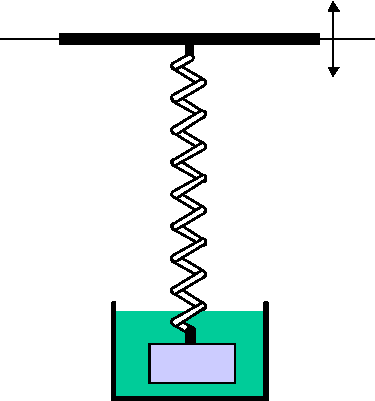
\includegraphics[width=\columnwidth, angle=90, origin=c]{images/spring_dashpot.pdf}}{
$x(t)=$ displacement from rest position\student{\subitem{$x=0 \Rightarrow$ no elastic  restoring force}}
\vfill
Newton's 2$^{nd}$ Law:\[ F = ma \qquad \text{where $a = \ddn{x}{t}{2}$}\]


}
\algn{F&=\text{sum of forces}\\&=\underbrace{\carray{\text{elastic restoring} \\ \text{force}}}_{\student{\carray{\text{Hooke's Law}\\=-kx }}} + \underbrace{\text{drag force}}_{\student{\carray{\text{opposes motion}\\ =-\beta\dd{x}{t}}}} + \quad \underbrace{\text{external forces}}_{\carray{\student{f(t)}}}\\
&= \student{-kx - \beta \dd{x}{t} +f(t)} }
}


\slide[Derivation of spring-dashpot ODE:]{
\twomini[.45]{.25}{.65}{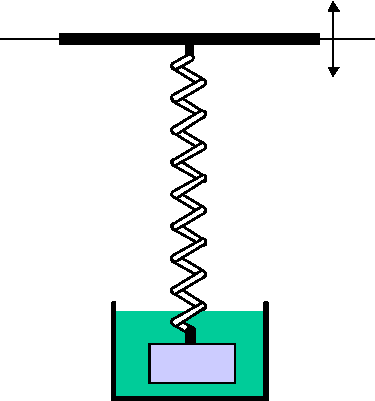
\includegraphics[width=\columnwidth, angle=90, origin=c]{images/spring_dashpot.pdf}}{
$x(t)=$ displacement from rest position\subitem{$x=0 \Rightarrow$ no elastic  restoring force}
\vfill
Newton's 2$^{nd}$ Law:\[ F = ma \qquad \text{where $a = \ddn{x}{t}{2}$}\]


}
\algn{F&=-kx - \beta \dd{x}{t} +f(t) \\
\student{m \ddn{x}{t}{2}} &\student{= -kx - \beta \dd{x}{t} +f(t)}}

\student{\[\boxed{ m x\pp + \beta x\p  + kx=  f(t) }\]}
}

\slide[Adding a constant pre-stress:  $f(t) \rightarrow f_0+f(t)$ ]{
\twomini[.55]{.25}{.65}{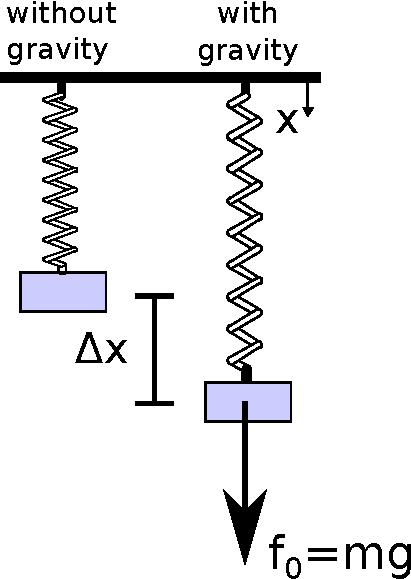
\includegraphics[width=\columnwidth]{images/spring_dashpot_gravity.pdf}}{\vspace{-1.5em}
\algn{mx\pp +\beta x\p +kx &= f_0 +  f(t)\intertext{Change of coordinate $\tilde{x} =  x-\frac{f_0}{k}$}
\student{m\tilde{x}\pp +\beta \tilde{x}\p +k\tilde{x} }&= \student{ f(t)}}\vspace{-1.5em}
\student{\subitem{$\tilde{x}=0 \Rightarrow$ restoring force + pre-stress = 0 \item $\tilde{x}$ = displacement from equilibirum position}}
\vfill
}
\itmz{\item Position dynamics do not change due to constant pre-stress.
\item Equilibrium position changes by $\Delta x = \frac{f_0}{k}$
\item Given $\Delta x$ and $f_0$ you can find $k=\frac{f_0}{\Delta x}$\vfill
\student{\subitem{e.x. $f_0=mg \Rightarrow k=\frac{mg}{\Delta x}$}}\vfill
}
}

\subsection{Simple Harmonic Motion}

\slide[Simple Harmonic Motion]{
Spring with no damping and no forcing, i.e. \[mx\pp+kx=0\]

\itmz{\item Similar: frictionless pendulum, circuit with no resistance….
\item General solution: \student{ 
Homogeneous problem
\algn{\text{Guess}: x(t)&=e^{rt} &mr^2e^{rt} +k e^{rt} &=0\\
&&mr^2+k&=0\\
r&=\pm\frac{\sqrt{-4km}}{2m}\quad =\pm i \sqrt{\frac{k}{m}}}
\[x(t)=c_1 \cos(\omega_0 t) + c_2 \sin(\omega_0 t); \qquad \omega_0=\sqrt{\nicefrac{k}{m}}\]
}
}
}

\slide[Simple Harmonic Motion:  $mx\pp+kx=0$ ]{

\itmz{
\item General solution:\[x(t) = c_1 \cos(\omega_0 t)  + c_2 \sin(\omega_0 t), \quad \omega_0 = \sqrt{\nicefrac{k}{m}} \]\vfill
\item All solutions have periodic motion with period: $T=\frac{2\pi}{\omega_0}$\vfill
\item The quantity $\omega_0$ is called the \student{\alert{natural frequency}.}\vfill
\item Obtaining a unique solution requires two initial conditions:
\student{\itmz{\item $x(0)$ = initial displacement away from rest position.\item $x\p(0)$ = initial velocity of the mass }}
}
}

\slide[Amplitude-phase form of solution:]{

\vfill Solution can also be expressed as \[x(t) = R \cos (\omega_0 t - \varphi)\]
\student{
\itmz{\item $R=$ amplitude of motion \subitem{max displacement}
\item $\varphi=$ phase angle \subitem{by convention $-\pi<\varphi<\pi$}}
}
\vfill
}

\slide[Amplitude-phase form of solution:]{\vspace{-2em}
\student{\algn{ \ucover{\text{Gen Solution:} \quad R\cos( \omega t -\varphi) } &\ucover{=\quad c_1\cos (\omega t)  \quad + \quad c_2\sin (\omega t)} \\
\ucover{\text{Trig ident:}\quad  R\cos( \omega t - \varphi)}  &\ucover{= R\left[ \cos \paren{ \omega t}\cos (\varphi) +\sin \paren{ \omega t }\sin (\varphi)   \right]} \\\\
\intertext{by visual inspection} R\cos \varphi &= c_1 &(1)\\
R\sin \varphi &= c_2 &(2)
}
\vfill
\twomini{.5}{.5}{$(2)/(1)$: \algn{\frac{R \sin \varphi}{R\cos\varphi}=\tan \varphi &=\frac{c_2}{c_1}\\
\Rightarrow  \Aboxed{\varphi = \arctan \paren{\frac{c_2}{c_1}}}}
}{$(1)^2+(2)^2$:
\algn{R^2\underbrace{(\cos^2 \varphi +\sin^2 \varphi)}_{1}&=c_1^2+c_2^2\\R^2&=c_1^2+c_2^2\\\Aboxed{R&= \pm \sqrt{c_1^2+c_2^2}}}

\vspace{-.5em}
Check at $t=0$ to determine + or -
} 
}
}
\settoggle{covered}{false}
\slide{A spring has spring constant of 15 N/m. A mass of 3 kg is attached to the spring, and is then displaced from the equilibrium position by 1cm and released with a velocity of 14 cm/s at $t=0$. \\~\\
\enum{ \item  Find the  displacement for  $t>0$. 
\item Find the natural frequency, period, amplitude, and phase angle of motion. }\vspace{-1em}
\student{\algn{3 x\pp + 15 x &= 0 \\
x(t) &= c_1 \cos (\omega_0 t) +c_2 \sin (\omega_0 t)\\
w_0&=\sqrt{k/m} = \sqrt{15/3} = \sqrt{5}
\intertext{Initial Conditions:}
x(0) &=  0.01 \text{m} = c_1\\
x'(0)  & = 0.14 \text{m/s} = \omega_0 c_2 =\sqrt{5} c_2\\
c_2&=\frac{0.14}{\sqrt{5}}
}
}
}

\slide{
\student{
\[\boxed{x(t) = 0.01 \cos{\sqrt{5} t } +  \frac{0.14}{\sqrt{5}} \sin{\sqrt{5} t}}\]
Amplitude and phase angle
\[x(t) = R\cos (\omega_0 t - \phi)\]

\algn{R &=\sqrt{c_1^2 +c_2^2} & \varphi & = \arctan\left({\frac{c_2}{c_1}}\right)\\
&=\sqrt{0.01^2+\frac{0.14^2}{5}} & &= \arctan{\left(\frac{14}{\sqrt{5}}\right)}\\
&\approx 0.0626 & &\approx 1.412\\\\
x(t)&\approx0.0626\cos \left(\frac{ t}{\sqrt{5}} -1.412\right)
}

}
}
\subsection{Damped Dynamics}
\slide[Free oscillations with damping]{
\[x\pp +\beta x\p +kx = 0 \]
What happens for small and large $\beta$?
\student{
\itmz{ 
\item  $\beta \to 0$, no damping $\Rightarrow$ recover simple harmonic oscillations
\item  $\beta \to \infty$, infinite damping $\Rightarrow$ no oscillations
}
}\vfill
Characterisitc equation: $mr^2+\beta r +k =0$ has two roots
\student{\[ r_{1,2} = \frac{-\beta \pm \sqrt{\beta^2-4km}}{2m}\]
\vfill
Note: Since $\beta>0$, the real part of $r_{1,2}$ is always negative \\\centerline{ $\Rightarrow$ exponentially decaying solutions.}}
}

\slide[]{
\[ r_{1,2} = \frac{-\beta \pm \sqrt{\beta^2-4km}}{2m}\]
Three cases:\student{
\enum{
\item $\beta^2<4km$: roots are complex \subitem{exp * (sin + cos) solutions - \alert{underdamped} motion}\vfill
\item $\beta^2>4km$: roots distinct and real \subitem{(bi-exponential solutions) - \alert{overdamped} motion}
\vfill
\item $\beta^2=4km$: repeated real root \subitem{($e^{rt} + te^{rt}$ solutions) - \alert{critically damped} motion}
}
}
}

\slide[Underdamped Motion]{
General solution: \[x(t) = e^{-\frac{\beta}{2m}t}\left( c_1 \cos (\omega_1 t) + c_2 \sin (\omega_1 t)\right)\] where $\omega_1=\sqrt{\nicefrac{k}{m} -(\nicefrac{\beta}{2m})^2} \student{\leq \omega_0}$ \student{(damping slows the oscillations)}
\vfill
We can write this in amplitude-phase form \student{\[x(t) = e^{-\frac{\beta}{2m}t}R \cos (\omega_1 t - \varphi) \]}\vspace{-1.25em}
\itmz{
\item $e^{-\frac{\beta}{2m}t}R$ is the time-varying amplitude (or amplitude)
\item $\omega_1$ is called the quasi-frequency of motion
\subitem{ $T=\nicefrac{2\pi}{\omega_1}$ is the quasi-period of motion}
\item $\varphi$ is the phase angle of motion (or phase shift)
}
\student{Again,  we have \hfill  $\varphi = \arctan \paren{\dfrac{c_2}{c_1}}, \qquad R=\sqrt{c_1^2+c_2^2}$ \hfill}
} 


\slide{\alert{Overdamped Motion:}\\
General Solution: \[x(t)=c_1e^{r_1t}+c_2e^{r_2t}\] with $r_1<r_2<0$.\vfill

\alert{Critically-Damped:} \student{$\beta=2 \sqrt{k \cdot m}$}\\
General Solution: \[x(t)=c_1e^{rt}+c_2te^{rt}\] with $r=\frac{-\beta}{2m}=-\sqrt{\nicefrac{k}{m}}<0$.\vfill

}



\slide{A spring has spring constant of 15 N/m. A mass of 3 kg is attached to the spring, and is then displaced from the equilibrium position by 3cm and released with an initial velocity of 0 cm/s  at $t=0$. \\~\\
\enum{ \item  Determine the value of the damping consant $\beta$ for which the system is critically damped.
\item Find the displacement $x(t)$ of the mass if the system is critically damped, assuming an inital velocity of 0 cm/s.}
}

\slide{A spring has spring constant of 15 N/m. A mass of 3 kg is attached to the spring, and is then displaced from the equilibrium position by 3cm and released with an initial velocity of 0 cm/s  at $t=0$. \\~\\
\enum{ \item  Determine the value of the damping consant $\beta$ for which the system is critically damped.
}\vfill
\student{\algn{\text{Critical damping:} \quad \beta^2 &= 4km\\&=4\cdot 3 \cdot 15=180\\
\beta &=\sqrt{180}\approx 13.416}}\vfill
}


\slide{A spring has spring constant of 15 N/m. A mass of 3 kg is attached to the spring, is then displaced from the equilibrium position by 3cm and released with an initial velocity of 0 cm/s  at $t=0$. \\~\\
\enum{ \setcounter{enumi}{1} \item Find the displacement $x(t)$ of the mass if the system is critically damped, assuming an inital velocity of 0 cm/s.
}
\student{\algn{x(t) &= c_1 e^{-\sqrt{\frac{k}{m}}t} +c_2 t e^{-\sqrt{\frac{k}{m}}t}= c_1 e^{-\sqrt{5}t} +c_2 t e^{-\sqrt{5}t}\\ \intertext{Initial conditions:}
x(0) &= 0.03 \text{m}  =  c_1\\
x\p(0) & = 0 = -\sqrt{5} c_1 + c_2 \left( 1 - \sqrt{5}\cdot 0  \cdot 1\right) = -\sqrt{5} c_1 + c_2\\
c_2 &= \sqrt{5} c_1 = \sqrt{5}\cdot  0.03 \approx 0.067 \\
x(t) &= 0.03 e^{-\sqrt{5}t} + 0.067t e^{-\sqrt{5}t}
}
}
}

\end{document}